\begin{savequote}[75mm] 
La verdad no penetra en un entendimiento rebelde. Si todos los lugares de la tierra est\'{a}n en el Aleph, ah\'{i} estar\'{a}n todas las luminarias, todas las l\'{a}mparas, todos los veneros de luz.
\qauthor{Jorge Luis Borges, El Aleph} 
\end{savequote}

\chapter{Integration of Information in Bioinformatics} \label{section:integration}


\begin{description}
	\item[First author publications]:\\
		\begin{enumerate}
			\item \label{paper:mydas} \bibentry{SAL2012}
			\item \label{paper:writeback}\bibentry{SAL2011}
			\item \label{paper:msctheses}\bibentry{SAL2010}
%			\item Gustavo A. Salazar et al. \emph{MyDas, an Extensible Java DAS Server} \emph{PLoS ONE} 2012, 7(9): e44180. doi: 10.1371/journal.pone.0044180
%			\item Gustavo A. Salazar et al. \emph{DAS Writeback: A Collaborative Annotation System} In \emph{BMC Bioinformatics} 2011, 12:143  doi:10.1186/1471-2105-12-143
		\end{enumerate}
 	\item[Coauthor publications]:\\
		\begin{enumerate}
			\setcounter{enumi}{3}
			\item \label{paper:dasty3} \bibentry{VIL2011}
			\item \label{paper:mykaryoview} \bibentry{JIM2011}
%			\item Jose M. Villaveces et al. \emph{Dasty3, a WEB framework for DAS} in  \emph{Bioinformatics}  2011, 27 (18): 2616-2617.
%			\item Rafael C. Jimenez et al. \emph{myKaryoView: A Light-Weight Client for Visualization of Genomic Data. } In \emph{PLoS ONE} 2011, 6(10): e26345. doi: 10.1371/journal.pone.0026345
		\end{enumerate}

	\item[Author's Contibutions]:\\
		\begin{itemize}
			\item \emph{\ref{paper:mydas}}: Conceived and designed the experiments: GS. Performed the experiments: GS AJ. Wrote the paper: GA LG PJ RJ. Critical revision of the manuscript for important intellectual input: RJ AQ AJ NM MM SH HH. Technical and material support: AJ NM MM SH HH. Supervision: NM MM SH HH. Study concept: GS LG PJ AQ RJ HH. Architectural design: PJ GS. Software development: GS LG PJ AQ. Evaluation of the compatibility with DAS protocol: AJ.
			\item \emph{\ref{paper:writeback}}: Critical revision of the manuscript for important intellectual input: RJ, AG, HH, NM and EB. Technical and material support: HH, NM and EB. Study supervision: HH, NM and EB. Study concept: GS, RJ and AG. Architectural design: GS and EB. Software development: GS. Drafting of the manuscript: GS. Design of the usability experiment: GS, NM and EB. All authors read and approved the final manuscript.
			\item \emph{\ref{paper:msctheses}}: MSc theses by GS, Supervision by EB, Co-supervision by NM
			\item \emph{\ref{paper:dasty3}}: Critical revision of the manuscript for important intellectual input: JV, RJ LG,GS, BG, NM, MM, AG and HH. Technical and material support: HH, NM, AG and MM. Study supervision: HH, NM, AG and MM. Study concept:  RJ and HH. Architectural design: JV, GS, BG and JG. Software development: JV. Drafting of the manuscript: JV, AG and LG. All authors read and approved the final manuscript.
			\item \emph{\ref{paper:mykaryoview}}: Conceived and designed the experiments: RCJ MC NM JD. Performed the experiments: RCJ MC. Analyzed the data: MC. Contributed reagents/materials/analysis tools: GS BG. Wrote the paper: MC.
		\end{itemize}
\end{description}
\newpage


\newthought{The data analysed in bioinformatics comes from diverse and heterogeneous sources}, for example, the data might be captured from wet-lab experiments or deduced with \emph{in-silico} procedures, it can refer to nucleic information and sequenced data, but also to expression levels and other protein information, it is possible to analyse isolated organisms or to gather information from multiple species. It all depends on the purpose of the research and the availability of data, however it is almost inevitable to have to integrate more than one of this sources in order to tackle todays research challenges.

This chapter is focused on the contributions done during this PhD in order to integrate data using the Distributed Annotation System. The first section describes  MyDas, a server tool that facilitate the publishing of DAS sources. A proposal to extend DAS in order to support collaborative annotation is described in section \ref{section:writeback}. We have grouped our participation in several client-side projects with DAS in the section \ref{section:dasvisual}. Lastly we will discussed the impact of this projects, together with the present and future of DAS.


\section{MyDas} \label{section:mydas}

The research of this section has been published in the paper \cite{SAL2012}, referenced as \ref{paper:mydas}, in the beginning of this chapter. 
Authors of this paper are Gustavo A. Salazar, Leyla J. García and Philip Jones (first authors); the co-authors provided input in line with their roles as supervisors.  Parts of this section are based on the work of collaborators and this is indicated clearly below. 

The contributions on the software development process of MyDas are as follow: The first version of the project was developed by Philip Jones with the collaboration of Anthony Quinn for the XSLT component. A second development cycle together with the support of the DAS version 1.6 was executed by Gustavo A. Salazar. Current maintenance of the software is lead by Leyla J. García. As an open source project, it has received contributions from other developers, but the mentioned authors here have been the leaders the project during its different stages.

\subsection{Overview}

There were over 1500 sources registered in the DAS registry by January 2015, and although not all of them implement the same capabilities, they all follow the DAS protocol,with almost half of them updated to the latest version DAS 1.6E. There are common tasks among DAS sources:  parsing, capture of arguments, exception handling, XML creation, dealing with the HTTP protocol, and more. And therefore a software specialised in these tasks is needed in order to allow a data providers to focus in their specific cases.

MyDas is a software product that assists in the process of publishing biological data through the DAS protocol. Data providers are asked to implement an adaptor that connects the logic of MyDas with the data itself, and from there MyDas executes all the HTTP interfaces, XML encodings and other required operations to support all the DAS capabilities.

In the following sections we describe the architecture of MyDas, and present some examples of existing DAS services built upon MyDas.

\subsection{ Design and Implementation}
MyDas is a Java Servlet Application accepting HTTP requests, typically with one request for each command in the DAS specification. Responses are valid XML documents. MyDas is a Java 1.6 application, and it runs on a Java servlet container such as Tomcat (\url{http://tomcat.apache.org/}) or Jetty (\url{http://jetty.codehaus.org/jetty/}). 

The development process of MyDas is supported by several tools, for example, it uses Maven (\url{http://maven.apache.org/}) for automatising the built, control of dependencies, test and deployment, it also uses JUnit (\url{http://www.junit.org}) in order to create a set of unit tests to ensure the quality of the software. Software workers are implemented on the repository machine, to execute the tests when new commits are submitted; notifying the main developers in case of failure.

\begin{figure}[t]
\centering
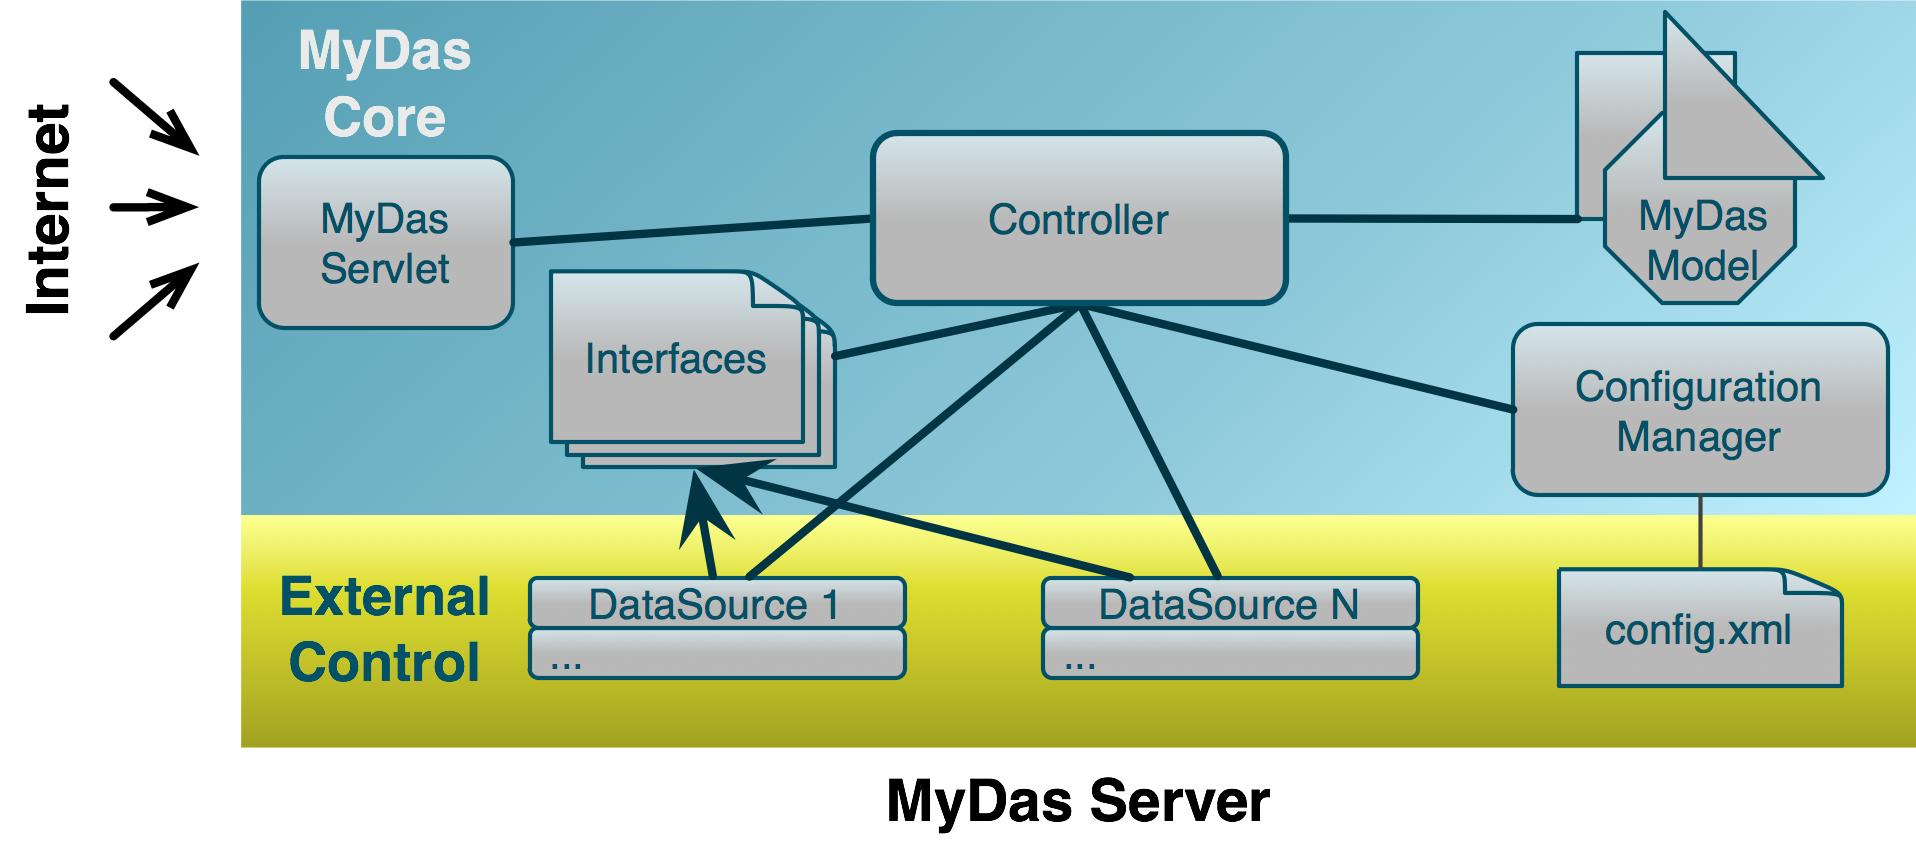
\includegraphics[width=\textwidth]{figures/MydasArchitecture.png}
\caption[MyDas Architecture.] {MyDas Architecture. The requesters can interact with MyDas through the servlet, which communicates the commands to the Controller. The Controller knows which Data Sources have been implemented by querying the Configuration Manager. Data Sources should implement at least one of the provided Interfaces. MyDas internally implements the DAS model.
\label{fig:mydas}}
\end{figure}

Figure \ref{fig:mydas} illustrates the architecture of MyDas, which is clearly divided between core and external control, in order to indicate what is offered by a blank installation of MyDas and what needs to be inputed by the data provider, for instance, its storage system (e.g. a relational database or flat file),  the strategy used to query the data (e.g. in-memory or using pre-indexing), etc.

Most of this information should be described in the configuration file, including data such as the URI, title, the relative path to the data source adapter. And then, the configuration manager makes the user options available to both the MyDas core and the data source implementation. 

The elements of the DAS specification have been mapped into a Java object model. Which must be used by the data source developer when creating an adapter. That is the way how the core of Mydas can use the same subroutines to deploy heterogeneous data into DAS. 

In order to facilitate the implementation of data sources, a template project is available, with examples of both reference and annotation servers: \url{https://code.google.com/p/mydas/downloads/detail?name=MyDasTemplate-1.6.7.zip}.

\subsection{Instances}
MyDas is being adopted by different data providers, including UniProt, InterPro and PRIDE.

UniProt (Universal Protein Resource)\cite{UNI2011} is a comprehensive catalogue of protein sequences and functional information. It consists of different databases, each optimized for different uses. The UniProt Knowledgebase (UniProtKB) is an expertly curated database providing a central access point for integrated protein sequence information. The UniProt Archive (UniParc) is a non-redundant sequence repository of all publicly available protein sequences. UniProt DAS (\url{http://www.ebi.ac.uk/das-srv/uniprot/das/uniprot}, \url{http://www.ebi.ac.uk/das-srv/uniprot/das/uniparc}) acts as a reference and annotation server, providing access to up-to-date information and allowing queries by UniProtKB and UniParc accessions numbers. There are currently more than 50 Data Sources that use UniProt DAS as a reference.

The InterPro database of predictive protein signatures is used for the classification and automatic annotation of proteins and genomes \cite{HUN2009}. InterPro provides several DAS data sources: DS\_327 (\url{http://www.ebi.ac.uk/das-srv/interpro/das/InterPro} ) serves matches that have been calculated to the predictive models supplied by the InterPro member databases for all UniProtKB protein sequences.  DS\_1028 (\url{http://www.ebi.ac.uk/das-srv/interpro/das/InterPro-matches-overview}) serves these matches resolved to the InterPro entries that integrate the member database signatures (providing a compact summary view of the domains, families and sites predicted for each UniProtKB sequence), and finally DS\_1029 (\url{http://www.ebi.ac.uk/das-srv/interpro/das/InterPro-UniParc-matches}) serves matches to member database signatures that have been calculated for UniParc protein sequences.

PRIDE DAS 1.6 (\url{http://www.ebi.ac.uk/pride-das/das/}) provides protein and peptide identifications together with supporting mass spectrometry evidence \cite{VIZ2009}. The information from PRIDE has already been shared using BioMart\cite{KIN2011}, therefore the strategy used to make it public to the DAS community was to develop an adaptor using MyDas to take the information from this source.

\subsection{Tutorials}
We have develop a three tutorials for the use of MyDas that are accessible via web (\url{http://code.google.com/p/mydas/wiki/Tutorials}). The tutorial are classified for its level of difficulty: Beginner, Intermediate and Advanced. 

The first tutorial helps the user in the setup of the example data source, in which no programming is required, and is limited to installation and configuration of MyDas. The tutorial for intermediate level guides through the common scenario of having a text file with some annotations to be displayed in DAS, in this case some the user requires to program the parsing of the file and mapping of it into the model. The third tutorial explores the case of getting data from a database system, which is a common way to store/access data in bioinformatics environments; this tutorial requires not only programming in Java, but also understanding queries written in SQL .

The power of MyDas is revealed when used on large data sets with elaborate schemas as in the last tutorial. The example uses the freely available mysql database provided by Ensembl. There are over a hundred databases hosted on the Ensembl servers, and in this case we used the core set of tables for Homo sapiens (version 56\_37a), and restricted our search scope to some high level features (e.g. Chromosome, genes, transcript). 

Many institutions may have a similar setup, however schema, policies and software vary from place to place. Although exporting files (and using them to publish data)  is an option, it implies that changes in the database won't be reflected in the generated files. In contrast, MyDas can be set up to take the information directly from the database management system and therefore will always be up to date.

\begin{figure}[t]
\centering
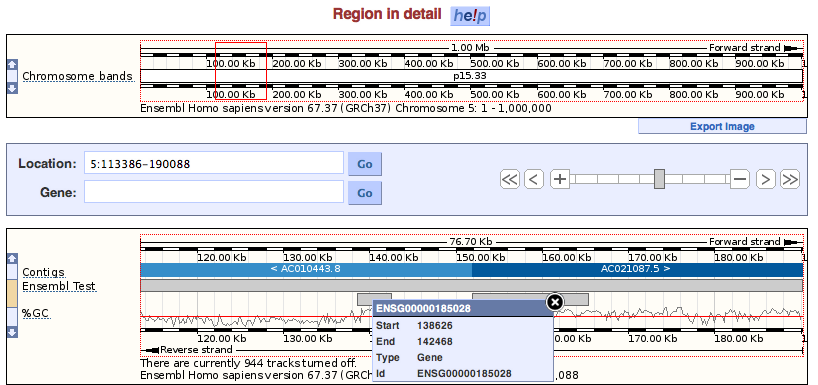
\includegraphics[width=\textwidth]{figures/MyDasEnsembl.png}
\caption[A MyDas Source as displayed on the Ensembl client.] {The data source created during the MyDas tutorials as it is visualised on the Ensembl web browser.
\label{fig:mydas_example}}
\end{figure}

A data source like this can be used by several tools to visualize its data. Figure \ref{fig:mydas_example} is a snapshot of the Ensembl browser, including the track named `Ensembl Test', whose information is obtained from the tutorial data source, demonstrating how the data published with MyDas can be displayed in well known genome browsers.

\subsection{Other DAS Servers}
The second tutorial mentioned above, describes the case where a user has a plain text file that follows a basic format (i.e. separated by a predefined character). This scenario is so common in bioinformatics that a software tool specialised in the publishing of this type of data have been built. easyDAS\cite{GEL2011}  is a preinstalled server, where a new data source can be configured by submitting a GFF file (or similar). This alternative is ideal for rapid publishing because it simplify tasks related with the hosting and storage of both data and server. The drawback is the lack of control over the data once it is deployed. 

\begin{table}[t]
	\begin{tabular}{|p{3cm}|p{2.7cm}|p{2.7cm}|p{2.7cm}|p{2.7cm}|}
\hline 
\emph{Feature} & \emph{MyDas} & \emph{ProServer} & \emph{Dazzle} & \emph{easyDAS}\\
\hline 
Language & Java & Perl & Java & Web App(Perl)\\
\hline 
Latest Release & 2011 & 2011 & 2010 & 2011\\
\hline 
DAS Version & 1.6 & 1.6 & 1.53E\footnotemark  & 1.6\\
\hline 
Physical Storage & Defined by User & Defined by User & Defined by User & Internal database\\
\hline 
Entity Responsible & EBI & Sanger Institute & Sanger Institute & EBI\\
\hline 
Main task to create a data source & Develop a Java class. & Develop a Perl adaptor & Develop a Java class & Submit a tabulated file.\\
\hline 
	\end{tabular}
	\caption{Features of the main DAS servers}
	\label{tab:table1}
\end{table}
\footnotetext{There is a branch of this project where capabilities of DAS 1.6 are been implemented, however there was not a stable version of it at the time of publishing.}

Besides MyDas there are other implementations of DAS servers such as Dazzle (\url{www.biojava.org/wiki/Dazzle}) or ProServer \cite{FIN2007},  amongst others (see \url{http://www.biodas.org/wiki/DAS/1#Implementation}). Nonetheless, MyDas and ProServer are the only servers that fully support the current DAS specification (1.6E). They differ from each other mainly in the language in which they are implemented (ProServer is written in Perl), but not in feature set, making system compatibility the major factor in deciding between the two.

Table \ref{tab:table1} summarizes some of the high level characteristics of the most well known DAS servers. 

We executed some benchmarking tests comparing MyDas, ProServer and Dazzle  in order to evaluate their loading performance. The test were ran through the Apache HTTP Server Benchmarking Tool (\url{http://httpd.apache.org/docs/2.0/programs/ab.html}).  was not taken into account for this test because it is installed on a different server, therefore there is no way to exclude network latency from the test.

The three server were installed in the same machine, creating data sources with the same data set in each of them. We prepared 3 DAS queries with expected responses of approximately 1.5Kb, 200Kb and 7.5Mb. Each query was repeated 1000 times with 10 concurrent connections

The 3 servers were able to complete all the requests and the table \ref{tab:table2} shows the main results of the executed test.

\begin{table}[!ht]
	\begin{tabular}{|p{6cm}|p{3cm}|p{3cm}|p{3cm}|}
\hline 
\emph{Figure} & \emph{MyDas} & \emph{ProServer} & \emph{Dazzle}\\
\hline 
Requests per Second - Mean (small) & 739.88 & 1.54 & 424.56\\
\hline 
Time per request - Mean (small) & 13.516 ms & 6492.978 ms & 23.554 ms\\
\hline 
Transfer Rate (small) & 1534.68 Kbytes/sec & 2.81 Kbytes/sec & 859.91 Kbytes/sec\\
\hline 
Requests per Second - Mean (medium) & 51.52 & 1.40 & 34.10\\
\hline 
Time per request - Mean (medium) & 194.114 ms & 7123.396 & 293.216 ms\\
\hline 
Transfer Rate (medium) & 10944.96 Kbytes/sec & 288.19 Kbytes/sec & 6997.52 Kbytes/sec\\
\hline 
Requests per Second - Mean (large) & 1.79 & 0.32 & 1.10\\
\hline 
Time per request - Mean (large) & 5589.148 ms & 30942.590 ms & 9110.292 ms\\
\hline 
Transfer Rate (large) & 13088.38 Kbytes/sec & 2283.04 Kbytes/sec & 7770.29 Kbytes/sec\\
\hline 
	\end{tabular}
	\caption{Benchmarking between the main DAS servers}
	\label{tab:table2}
\end{table}

This comparison can not be conclusive in deciding the best or fastest DAS server, mainly because each data source has unique challenges and different cases can generate different results. Nonetheless, given that the three servers provide a data source implementation to publish data from a GFF file, they were configured to use the same GFF file to ensure equal conditions. 

The figures in the table show that in all 3 scenarios MyDas performed better than the other servers. It is important to note that both MyDas and Dazzle were running on the same Tomcat server, therefore the conditions for both were the same. ProServer on the other hand, is a standalone server that implements socket communications in the application itself, which is an advantage in terms of making it easy to use.

The complete results of the tests are available in Appendix \ref{ap:stress}.










%\newpage
\section{DAS Writeback}\label{section:writeback}

Large part of the work included in this section was executed prior the timeframe of this PhD during the MSc referenced as No. \ref{paper:msctheses} at the beginning of this chapter. Nonetheless, the inclusion of this contribution in this document is relevant because the software was reengineered as part of this PhD, upgrading it to the latest DAS specification and using the most recent versions of its dependencies: MyDas and Dasty3. The results of both MSc and reengineering process were published in \ref{paper:writeback} as reported at the top of this chapter, which author is Gustavo A. Salazar and the co-authors provided input in line with their roles as collaborators and supervisors. 

\subsection{Overview}
DAS offers a uniform protocol to share data that can, and has been used, for diverse data providers. One of the advantages of this approach is that users now can collect information from multiple resources by using a single tool. However we consider that opening the communication in the opposite direction (i.e. users submitting annotations to the resources), is a desirable functionality that was not included in the firsts versions of the protocol.

For example, researchers using a DAS client to gather information of a protein of their interest, can notice errors on current features, or missing annotations. It is unrealistic to expect such user to deploy a DAS source to publish a handful of annotations. The traditional alternative is for them to report the new features to the providers. This however takes time, and falls into the inconveniences of having a centralised repository, where the user might have to wait for the release of a new version of the data before it can actually use it in the client.

As a solution to this problem, we have designed and implemented the Distributed Annotation System (DAS) Writeback, which enables community-based manual annotation of public data. Our approach makes the process of manual annotation a collaborative task, whereby any individual can participate by sharing their knowledge in the form of new or edited annotations.

The DAS Writeback system provides the capabilities of reading, writing, editing and deleting features by users of a web application. For the design and development of such a system it was necessary to model an architecture that supports the new features, define an extension of the DAS specification to accommodate the client-server communication, and implement server and client components. All of these milestones were achieved while trying to follow the same style as the existing DAS technology, thus looking for an easy adoption of the system by the DAS community.

\subsection{DAS as RESTful services}
The strategy used to define the architecture of a writeback system for DAS, was to conciliate two technical concepts: one the one hand, DAS uses the REST protocol for web services \cite{PRL2007}, and on the other hand, reading and writing functionalities have been widely explore in Relational DataBases Management Systems (RDBMS), where the basic operations are  known as CRUD (Create, Read, Update and Delete) \cite{KIL1990}.

One of the major strengths of the RESTful strategy is that it is based on such widely adopted standards as HTTP, XML, URI and MIME. This makes REST, and therefore DAS, technologies easy to implement and attractive to both developers and final users. Considering this we decide that when extending the DAS protocol to support servers that can store edited annotations, we set out to retain compatibility with the existing read-only system of HTTP GET requests. 

One of the main features of the REST architecture is to have a uniform interface. This means that REST resources should be manipulated using a predefined set of operations. In the case of the Web, those operations are the 4 basic reading/writing operations CRUD, and the HTTP methods PUT, GET, POST and DELETE are suggested in the literature to specify those actions. These operations \textit{``are broadly applicable but they also help uphold specific Web architectural properties''} \cite{VIN2008}.

The DAS specification in its version 1.53E it is well detailed in the implementation of the reading and querying capabilities of the system, this however only cover the use of the GET, and there is no mention of any of the other RESTful methods.

Our proposal is to extend the DAS protocol in order to define the use of the other RESTful methods to complete the inclusion of the CRUD functionalities into the DAS system, and consequently, provide the DAS community with the appropriate tools for collaborative annotation.

A previous effort in a similar direction was the object of a MSc thesis, where a DAS Writeback server was developed as a proof of concept \cite{GRZ2008}, however it used different technologies and it wasn't closely attached to the RESTful protocol, which are factors that we consider to be key in the adoption of any extension on DAS.

\subsection{Architecture}
The components of the system were developed bearing the following goals in mind:
\begin{enumerate}
\setlength\itemsep{-0.5em}
\item The original annotations of a DAS source should not be modified directly.
\item The system should be trusted by the user.
\item The system should promote interaction between the server and users.
\end{enumerate}

The first goal has been established in order to ensure that the data shared by a provider is not in risk of been changed or deleted by any case of vandalism or by mistake when using the write back system. In order to do this, the architecture includes a third party writeback server that stores the changes to a set of annotation, independent of the original source providing those annotations. 

New features, editions and deletions are saved in the writeback server as annotations themselves and therefore they can be in turn be edited or deleted, by other users. We hope that this feature, gives the users the sense of trust (goal 2) that other collaborative systems such wiki projects have, where the community ensures the quality of the information. 

Finally on a way to promote the use of the writeback system we implemented the functionalities on the well known protein DAS client Dasty. With the objective of bringing the new functions on a system users were already familiar with.

\begin{figure}[ht] 
\centering
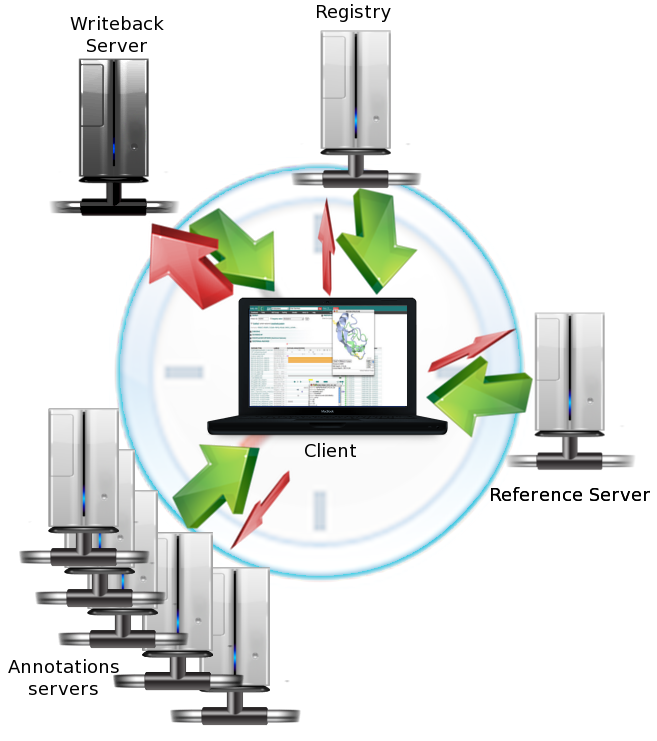
\includegraphics[width=4in]{figures/WritebackArchitecture.png} 
\caption[Writeback in the DAS Architecture]{\emph{Writeback in the DAS Architecture}: Extension of the DAS architecture for the writeback. A third party writeback server is the last to be queried by the client, and its response is used to update the information provided by the annotation servers. Communication with the writeback server has the peculiarity that the amount of information sent by the client is considerably larger than for any other server. The clock in the background represents the chronological order of the actions in a DAS transaction.}  \label{fig: WritebackArchitecture}
\end{figure}

Figure \ref{fig: WritebackArchitecture} represents the architecture of DAS including the writeback server. Firstly it is necessary to highlight that, when a feature is requested, the writeback server behaves as another annotation server, using the same DAS commands. The way this information is rendered is the responsibility of the client. 

A standard DAS transaction starts by querying the DAS Registry (the DAS Registry provides a repository for the registration and discovery of DAS services). Next the reference sequence is obtained, followed by parallel requests to several annotation sources. The interaction between client and writeback occurs after the client has retrieved and displayed all of the information for the target protein, since it is only then that the user has a complete landscape view to take the decision to add, update or delete a feature.

HTTP requests relating to write operations on the writeback server are much larger than standard DAS requests (shown in Figure \ref{fig: WritebackArchitecture} as the width of the red arrow). The reason for this is that the client is now required to send the information to add or update a specific feature, including its type, category, position and other characteristics predefined in DAS. The communication with the writeback server is thus extended beyond the display of a graphic that compiles the information from all the servers. This is when the user starts to interact with the information, transforming the client from a pure visualisation tool to an interactive interface between the user and the DAS data.





\subsection{Protocol Extension}
As described in \ref{ssec:DASprotocol}, the version 1.53 of the DAS protocol had its continuation on the 1.53E, in which a set of proposed extensions were included. The same schema was followed when version 1.6 was released shortly followed by 1.6E, in which was decided by the DAS community that new extensions can be proposed using the wiki page of the project (\url{http://www.biodas.org}), and its adoption will determine its inclusion as a core component on future versions.

We follow this directions in order to include the writeback into DAS, which eventually became the first official extension on DAS 1.6E. The proposed specification can be found on the DAS1.6E web page (\url{http://www.biodas.org/wiki/DAS1.6E\#DAS\_writeback}). It proposes that both input and output documents for the writeback should follow the DAS GFF format (See code below for an example); the HTTP method indicates what to do with the received document, the method GET is still been used for querying and reading while POST, PUT and DELETE should be use to create, update or delete a feature.

The HTTP status codes used for DAS remain valid and will indicate success or failure of the requested command (e.g. HTTP code 200 for success)

%\newpage
\begin{lstlisting}
<?xml version="1.0" standalone="no"?>
<DASGFF>
	<GFF>
		<SEGMENT id="P13569" start="1" stop="1480" version="f29b8c0a9056a0f7680f3290d259b6ac">
			<FEATURE id="new" label="ISFCSQFSWIMPGTIK">
				<TYPE id="Polypeptide" cvId="Polypeptide">Polypeptide</TYPE>
				<METHOD id="ECO:0000160" cvId="ECO:0000160">
					Inferred from protein separation followed by fragment identification
				</METHOD>
				<START>488</START>
				<END>503</END>
				<NOTE>note added in the writeback</NOTE>
				<NOTE>USER=username</NOTE>
				<NOTE>PASSWORD=password</NOTE>
			</FEATURE>
		</SEGMENT>
	</GFF>
</DASGFF>
\end{lstlisting}


\subsection{Implementation}
We have developed a DAS writeback tool by extending existing DAS clients and servers. The writeback is included as a plug-in of Dasty3 and is integrated in the latest implementation of MyDAS, compliant with the current DAS 1.6 specification. 

\subsubsection{Server}
Our implementation of DAS Writeback is an extension of the MyDAS server, which has been widely described in section \ref{section:mydas}. A writeback data source was implemented to store annotations. Annotations are the main entity in the data model, and any edits or deletions of an annotation are considered to be versions of the original annotation.

The datasource uses Hibernate \cite{BAU2006} as its layer to access the persistence data, which brings the advantage of being \emph{Database-Engine} independent. The data source has been successfully tested using PostgreSQL, MySQL and Derby but is expected to work properly in other engines.

\subsubsection{Client}
One of the goals of this project was to create the perception for users that the writeback functions in a client are native and can be used naturally with existing clients. For this reason, the extension of an existing client was preferable to implementing a new one from scratch. In addition, the writeback server behaves as any other DAS server for reading purposes, so many software routines of an existing client could potentially be reused for the writeback visualisation.

We decided to use Dasty for our first DAS writeback client and a prototype was developed for Dasty2 and is details about it can be found in \cite{SAL2010}. We collaborated in the development of some of the components of Dasty2 \cite{JIM2008} and the knowledge of the software influenced the decision of using it for the writeback.

Later, in 2010, Dasty2 went through a refactoring process, optimising its code to provide a plug-in framework. The new version is called Dasty3 and our collaboration in its development is described in section \ref{section:dasty}. The writeback client was rewritten as a plugin for Dasty3 and is included in its core feature set.

%The communication between writeback client and server is achieved using the DAS GFF XML format, which is defined in the DAS specification (See example code above). The client has a logical model to map the DAS GFF format when it is reading from the writeback server, and also starts from this model to build the XML when information is to be sent to the server.

%The extensions performed in Dasty3 in order to support the writeback capabilities are divided below into reading and writing functions, i.e. if annotations are requested or if a change/creation is submitted, respectively:

\subsubsection{CRUD functions}
Below we describe how the CRUD functions (i.e. Create, Read, Update, Delete) have been implemented in both client(Dasty3 plugin) and server(MyDas extension).

\begin{figure}[ht]
\centering
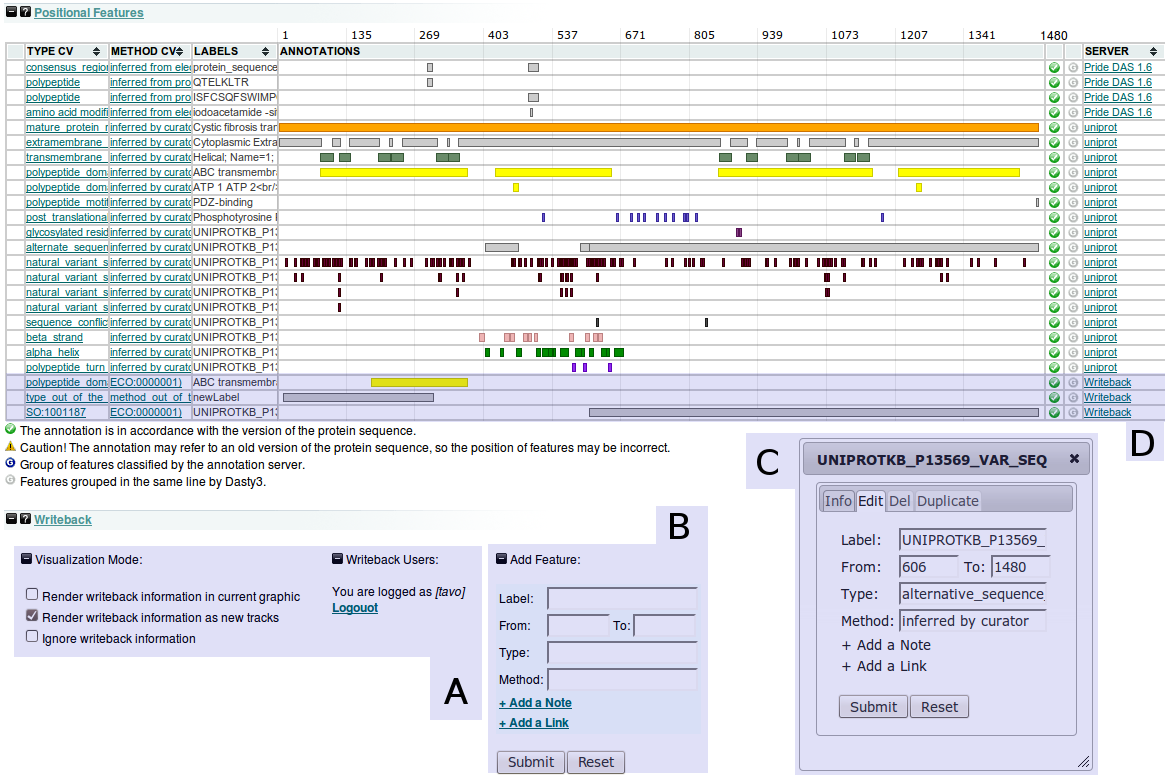
\includegraphics[width=6.5in]{figures/dasty3wbT.png} 
\caption{Dasty3+Writeback}  \label{fig: dasty+wb}
\end{figure}

\paragraph{Create}
Previous versions of MyDas were using GET and POST methods indistinctively, therefore the first modification done to the server was to identify the different HTTP methods and redirect the flow of data to its corresponding action. In order to create a new annotation, MyDas now listen to any POST method, and if its content is a GFF file its parsed and added to the data source. 

On the client side, a new form was added under the annotation graphic (\ref{fig: dasty+wb} B) in which the user can describe the new feature specifying label, location, type and evidence; notes and links are optional fields for the new feature. 

Version 1.6 of the DAS specification recommends the use of ontologies in order to standardise both types and evidence codes, and make the task of integrating annotation from several servers easier. In order to promote the use of those ontologies, a list of suggested terms from the corresponding ontology is displayed in the edit form.
  
\paragraph{Read}
The writeback server behaves like any other DAS source when a set of features is requested. The client decides when and how to process this information. For the Dasty3 writeback plug-in, the user has three different modes to operate (Figure \ref{fig: dasty+wb} A): (i) to ignore the writeback annotations, (ii) to use the writeback as any other annotation source, or (iii) to replace original annotations with the writeback information. The latter option generates a similar graphic for features as normally rendered by Dasty3, but incorporating the modifications that the writeback server contains. 

\paragraph{Update}
When a Dasty3 user clicks on a feature, a popup window with the complete information of the annotation is displayed. We have extended this functionality by including tabs on the popup window. The ``Edit'' tab contains a similar form as the one for a new feature, but it gets filled with the the information of the selected annotation (Figure {fig: dasty+wb} C). 

The information of this form is sent to the server using the method PUT, MyDas identifies the method, parses the GFF document and stores its content as the current version of the feature. The latest version will be the one to which the server returns for future requests.

\paragraph{Delete}
Del is nnother tab available in Dasty3 when a feature is selected. its content is just a confirmation dialog where the user expresses the desire of removing that feature. The DELETE HTTP method is then invoked, including the identifier for the feature. When MyDas detects a DELETE requests, it creates another annotation to register this command.  Which means that features are not really deleted from the server. The features tagged as deleted will be transparent in the Dasty3 graphic, and just its border will be visible.


\subsubsection{Other writeback functions}
A basic module to allow for user authentication through a login and password was added in the writeback panel (Figure \ref{fig: dasty+wb} A). Any writing function is conditional on prior login and password validation. The reading functionality does not require authentication.

Another way to edit a feature is through the history tab , In this window, the content of any previous version of the selected feature is displayed. In this case, the user can choose to roll-back to a previous version, and what actually happens is that a new edit request through the PUT HTTP method is submitted, therefore a rollback task does not removes the existing history, but rather adds a new edition to it.




	
\section{DAS Visualizations} \label{section:dasvisual}
\subsection{Dasty} \label{section:dasty}
The communication between the client and the writeback server has some differences with respect to the communication with other DAS servers. Firstly, the different HTTP methods (PUT, GET, POST and DELETE) should be used according to their function. For this reason, the proxy component of Dasty3 was extended to support the appropriate method usage. 

The second difference is in the amount of information transferred; before the writeback, all the requests in Dasty3 were using the \emph{GET} method. Therefore the information sent from the client to the proxy was limited to 256 characters, which is the URL size limit for some web browsers and servers. With the writeback functionalities, however, the client sends an XML document that is likely to exceed the URL size limit, making the use of other HTTP methods mandatory. This reinforces the applicability of the choice of adopting the RESTful standard. 

\subsection{myKaryoView}\label{section:mykarioview}
\subsection{probeSearcher}
\section{Discussion}
MyDas currently forms the basis for high volume DAS servers like UniProt and InterPro. It combines performance and stability with ease of installation, operation, and extension. The simplest way to run the server is to provide annotations in the form of a simple GFF file. At another level, the MyDas interface is efficient at implementing additional custom data sources, such as relational databases.

While the recently published easyDAS server provides a platform for DAS-based sharing of small sets of nucleic acid or protein annotations, and ProServer addresses Perl-based environments, MyDas offers a developer-friendly solution for laboratories and institutions that wish to share medium to large scale datasets in a Java-based environment. It completes the landscape of modern, open source DAS servers available to organisations sharing biomolecular data via the distributed DAS protocol. 

At the time of writing this manuscript, the DAS registry reports over 1200 data sources. This illustrates the high adoption of DAS, making it the perfect environment for a collaborative approach as presented here. The writeback specification is now an official extension in DAS and is considered to be a part of the core protocol. The developed software has been well received by the community. On the one hand, the server implementation is now part of the official development of one of the more stable DAS servers (myDas); and, on the other hand, the client is included in the set of plugins of Dasty3, which is a widely used DAS client. However, the success or failure of any collaborative system is recognized through the interaction of real users with the system, and additional time is required to be determine this. We hope this system will contribute to creation of a more publicly accessible, easily updatable, and reliable protein knowledge base.

The experiment vindicated our User Centered Approach. The one major issue has been corrected, and in general we demonstrated the usefulness of our concept. All the groups that participated in the experiment were able to Create/Update DAS annotations from a published paper, so we consider this to demonstrate that our system is effective, usable and will provide the appropriate environment for the creation and development of a protein annotation community.

